\appendix
\renewcommand{\chaptername}{Phụ lục}
\chapter{Các tham số trong Diffusion}
 \label{Appendix1}

\section{Sự thay đổi của $\sqrt{\alpha}$ và $\sqrt{1 - \alpha}$}

\setcounter{figure}{13}
\begin{figure}[H]
	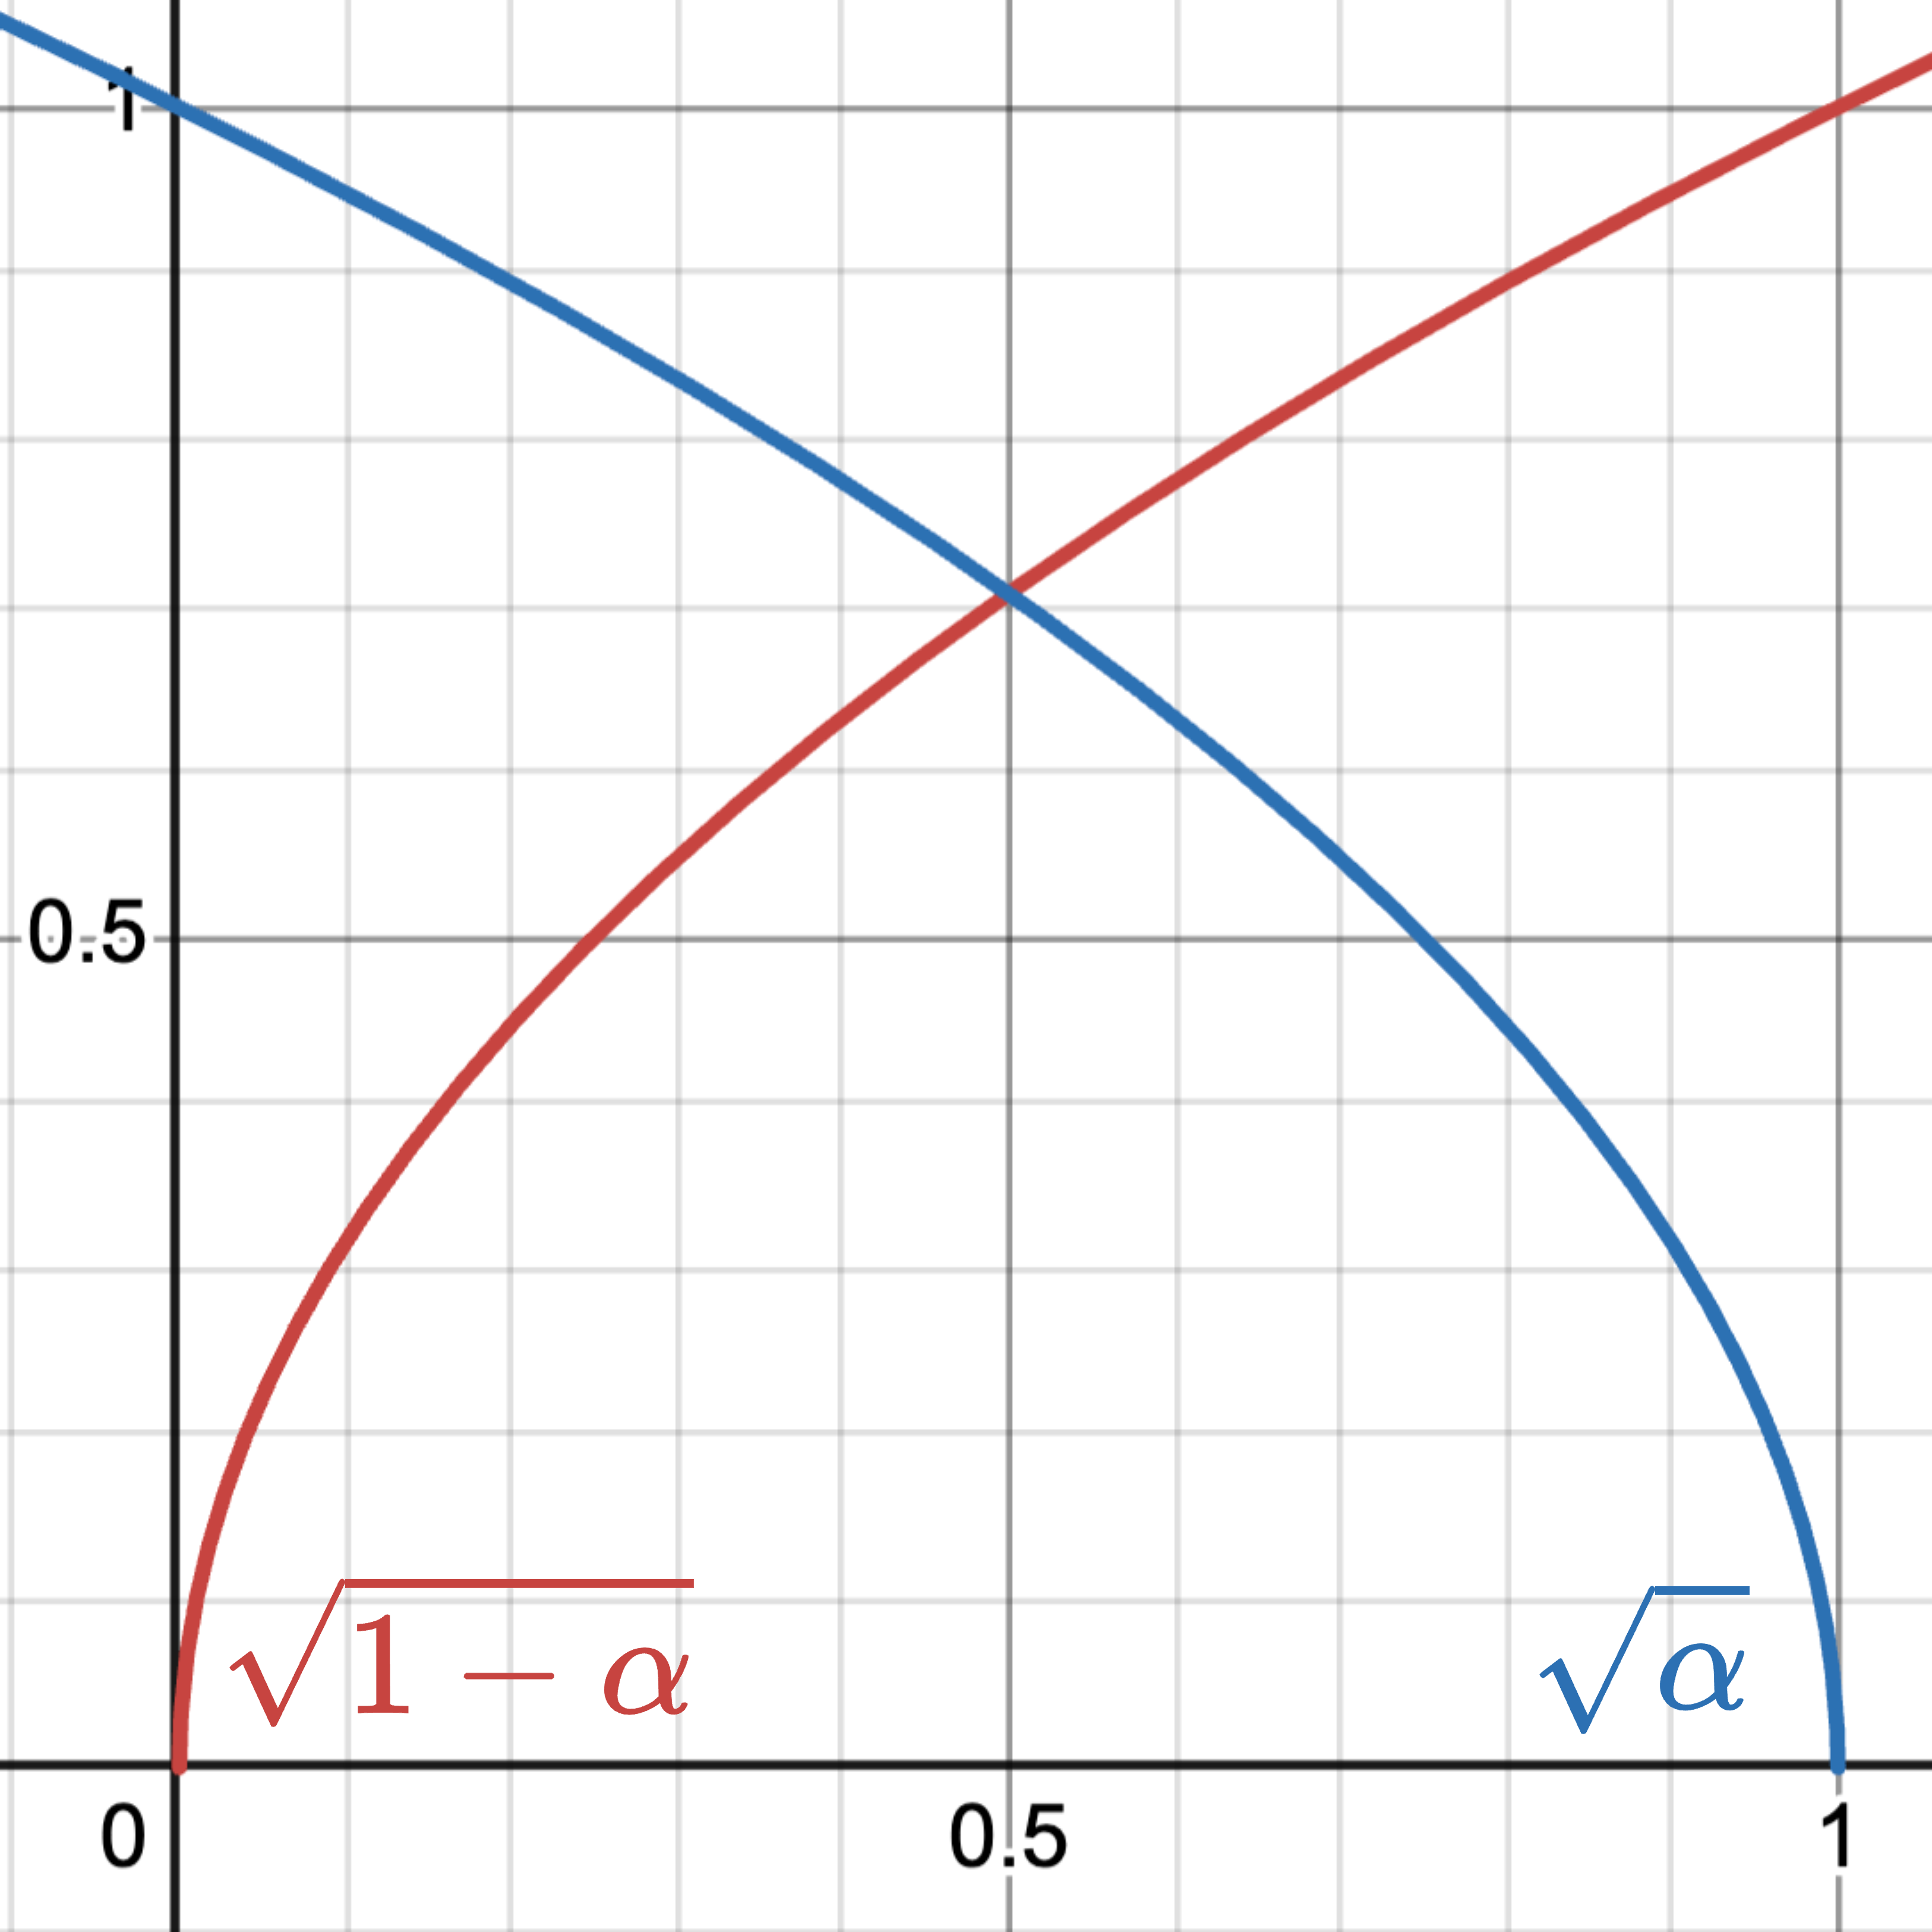
\includegraphics[width=0.5\linewidth]{SquareAlpha}
	\label{fig:wrapfig}
	\caption{Sự thay đổi của $\sqrt{\alpha}$ và $\sqrt{1 - \alpha}$}
\end{figure}

Trong quá trình diffusion, hệ thống muốn giảm dần sự hiện diện của $\bx$ và tăng dần sự hiện diện của nhiễu $\epsilon_t$. Với $\mathbf{x}_t = \sqrt{\alpha_t} \mathbf{x}_t + \sqrt{1 - \alpha_t} \epsilon_t$. Các hệ số $\sqrt{\alpha_t}$ và $\sqrt{1 - \alpha_t}$ giúp điều khiển quá trình này như sau:



\begin{itemize}
	\item $\sqrt{\alpha_t}$: Ban đầu giá trị lớn nhưng giảm dần để giảm sự ảnh hưởng vào kết quả tổng giữa nhiễu và $\bx_t$
	\item $\sqrt{1 - \alpha_t}$: Ban đầu giá trị nhỏ nhưng tăng dần theo từng bước. Với mục tiêu là đến cuối cùng thì sự ảnh hưởng của nhiễu càng lớn và trở thành nhiễu hoàn toàn.
\end{itemize}


Cả hai đại lượng này thay đổi theo thời gian trong quá trình diffusion, từ đó quyết định mức độ nhiễu được thêm vào từng bước $t$ và mức độ giữ lại trạng thái trước đó qua từng bước.


\section{Sự thay đổi của $\sqrt{\bar{\alpha}}$ và $\sqrt{1 - \bar{\alpha}}$}

$\bar{\alpha}_t = \prod_{i=1}^t \alpha_i$.  $\sqrt{1 - \bar{\alpha}_t} = \sqrt{1 - \prod_{i=1}^t \alpha_i}$. Cả $\sqrt{\bar{\alpha}}$ và $\sqrt{1 - \bar{\alpha}}$ đóng một vai trò quan trọng trong quá trình huấn luyện và sinh cử chỉ. Giúp kiểm soát mức độ nhiễu được thêm vào và cử chỉ, ta có thể thấy $\sqrt{\bar{\alpha}}$ giảm dần còn $\sqrt{1 - \bar{\alpha}}$ thì tăng dần..


\begin{figure}[H]
	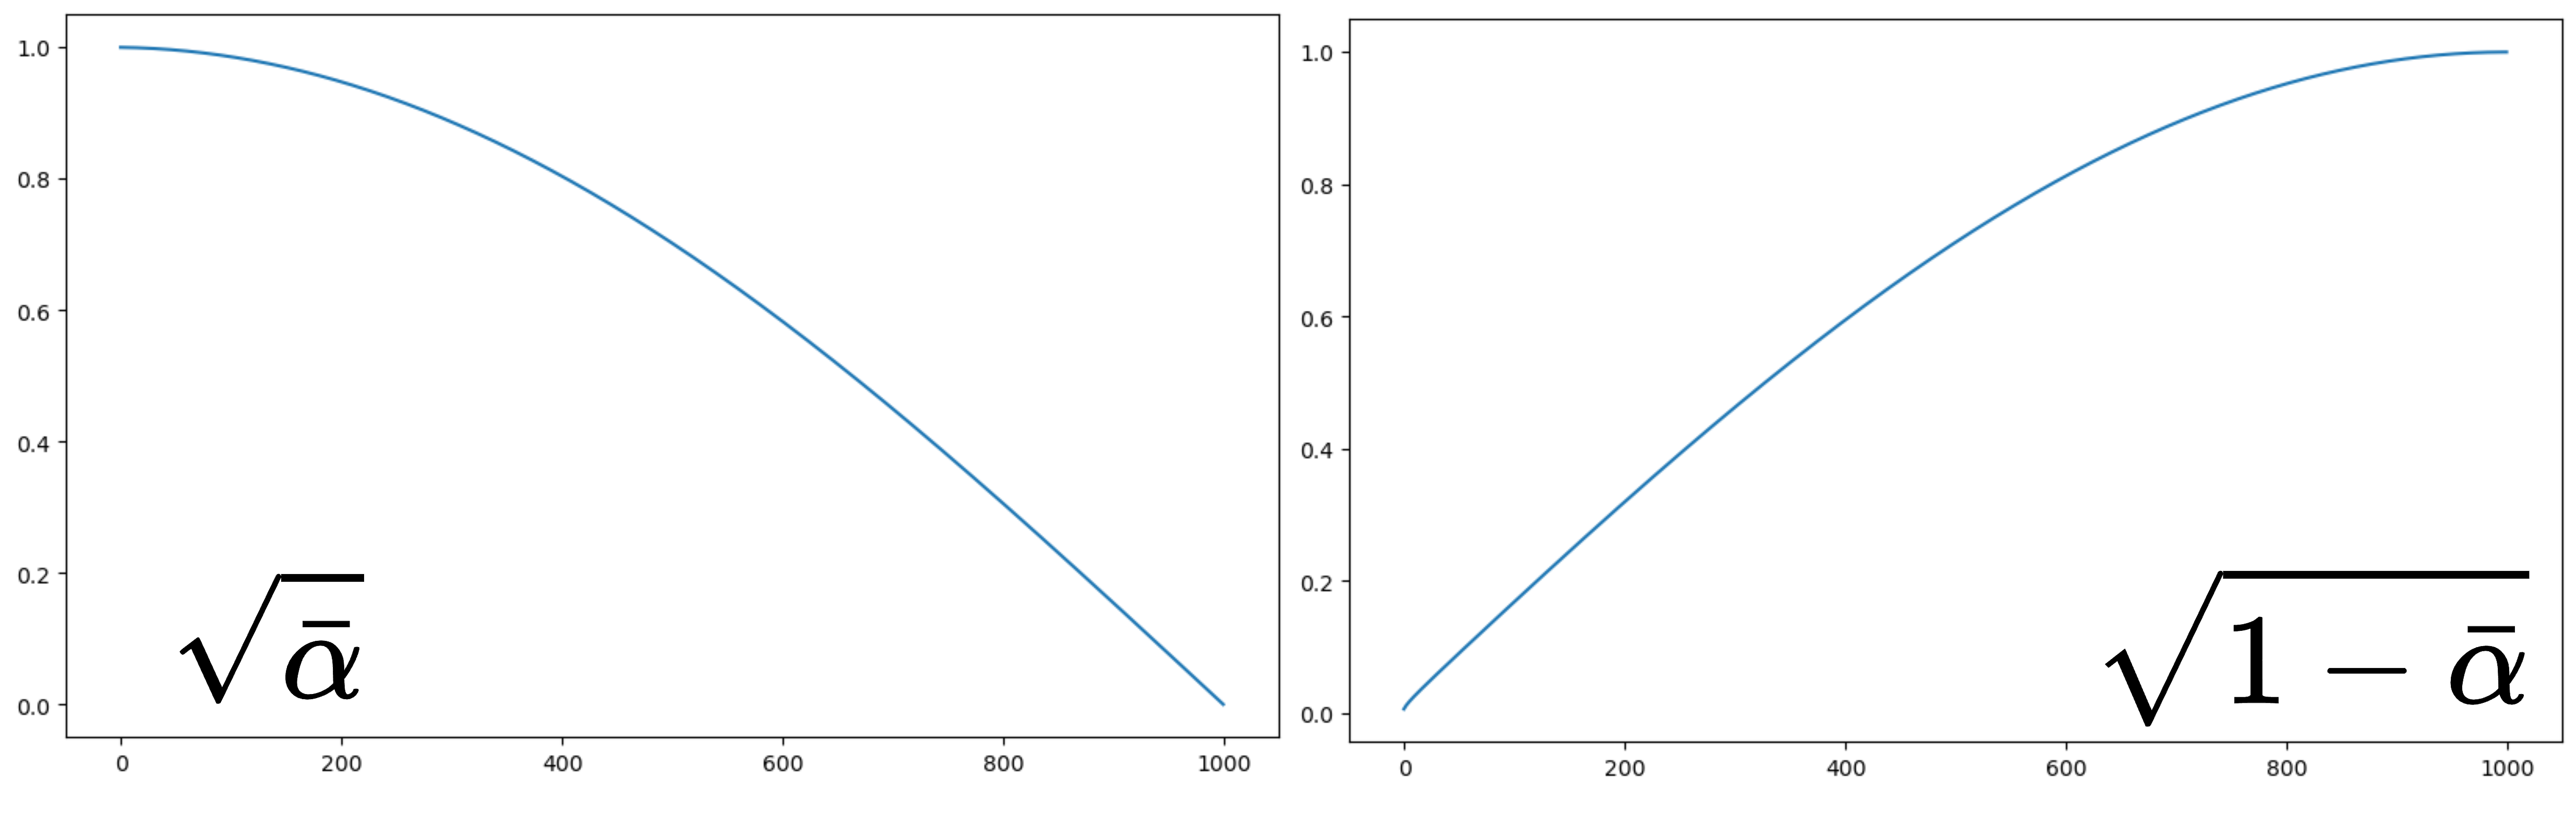
\includegraphics[width=\linewidth]{AlphaCumprod}
	\label{fig:AlphaCumprod}
	\caption{Quá trình thay đổi của $\sqrt{\bar{\alpha}}$ và $\sqrt{1 - \bar{\alpha}}$}
\end{figure}

\section{So sánh $\epsilon$ objective và  $\bx_0$ }

\begin{figure}[H]
	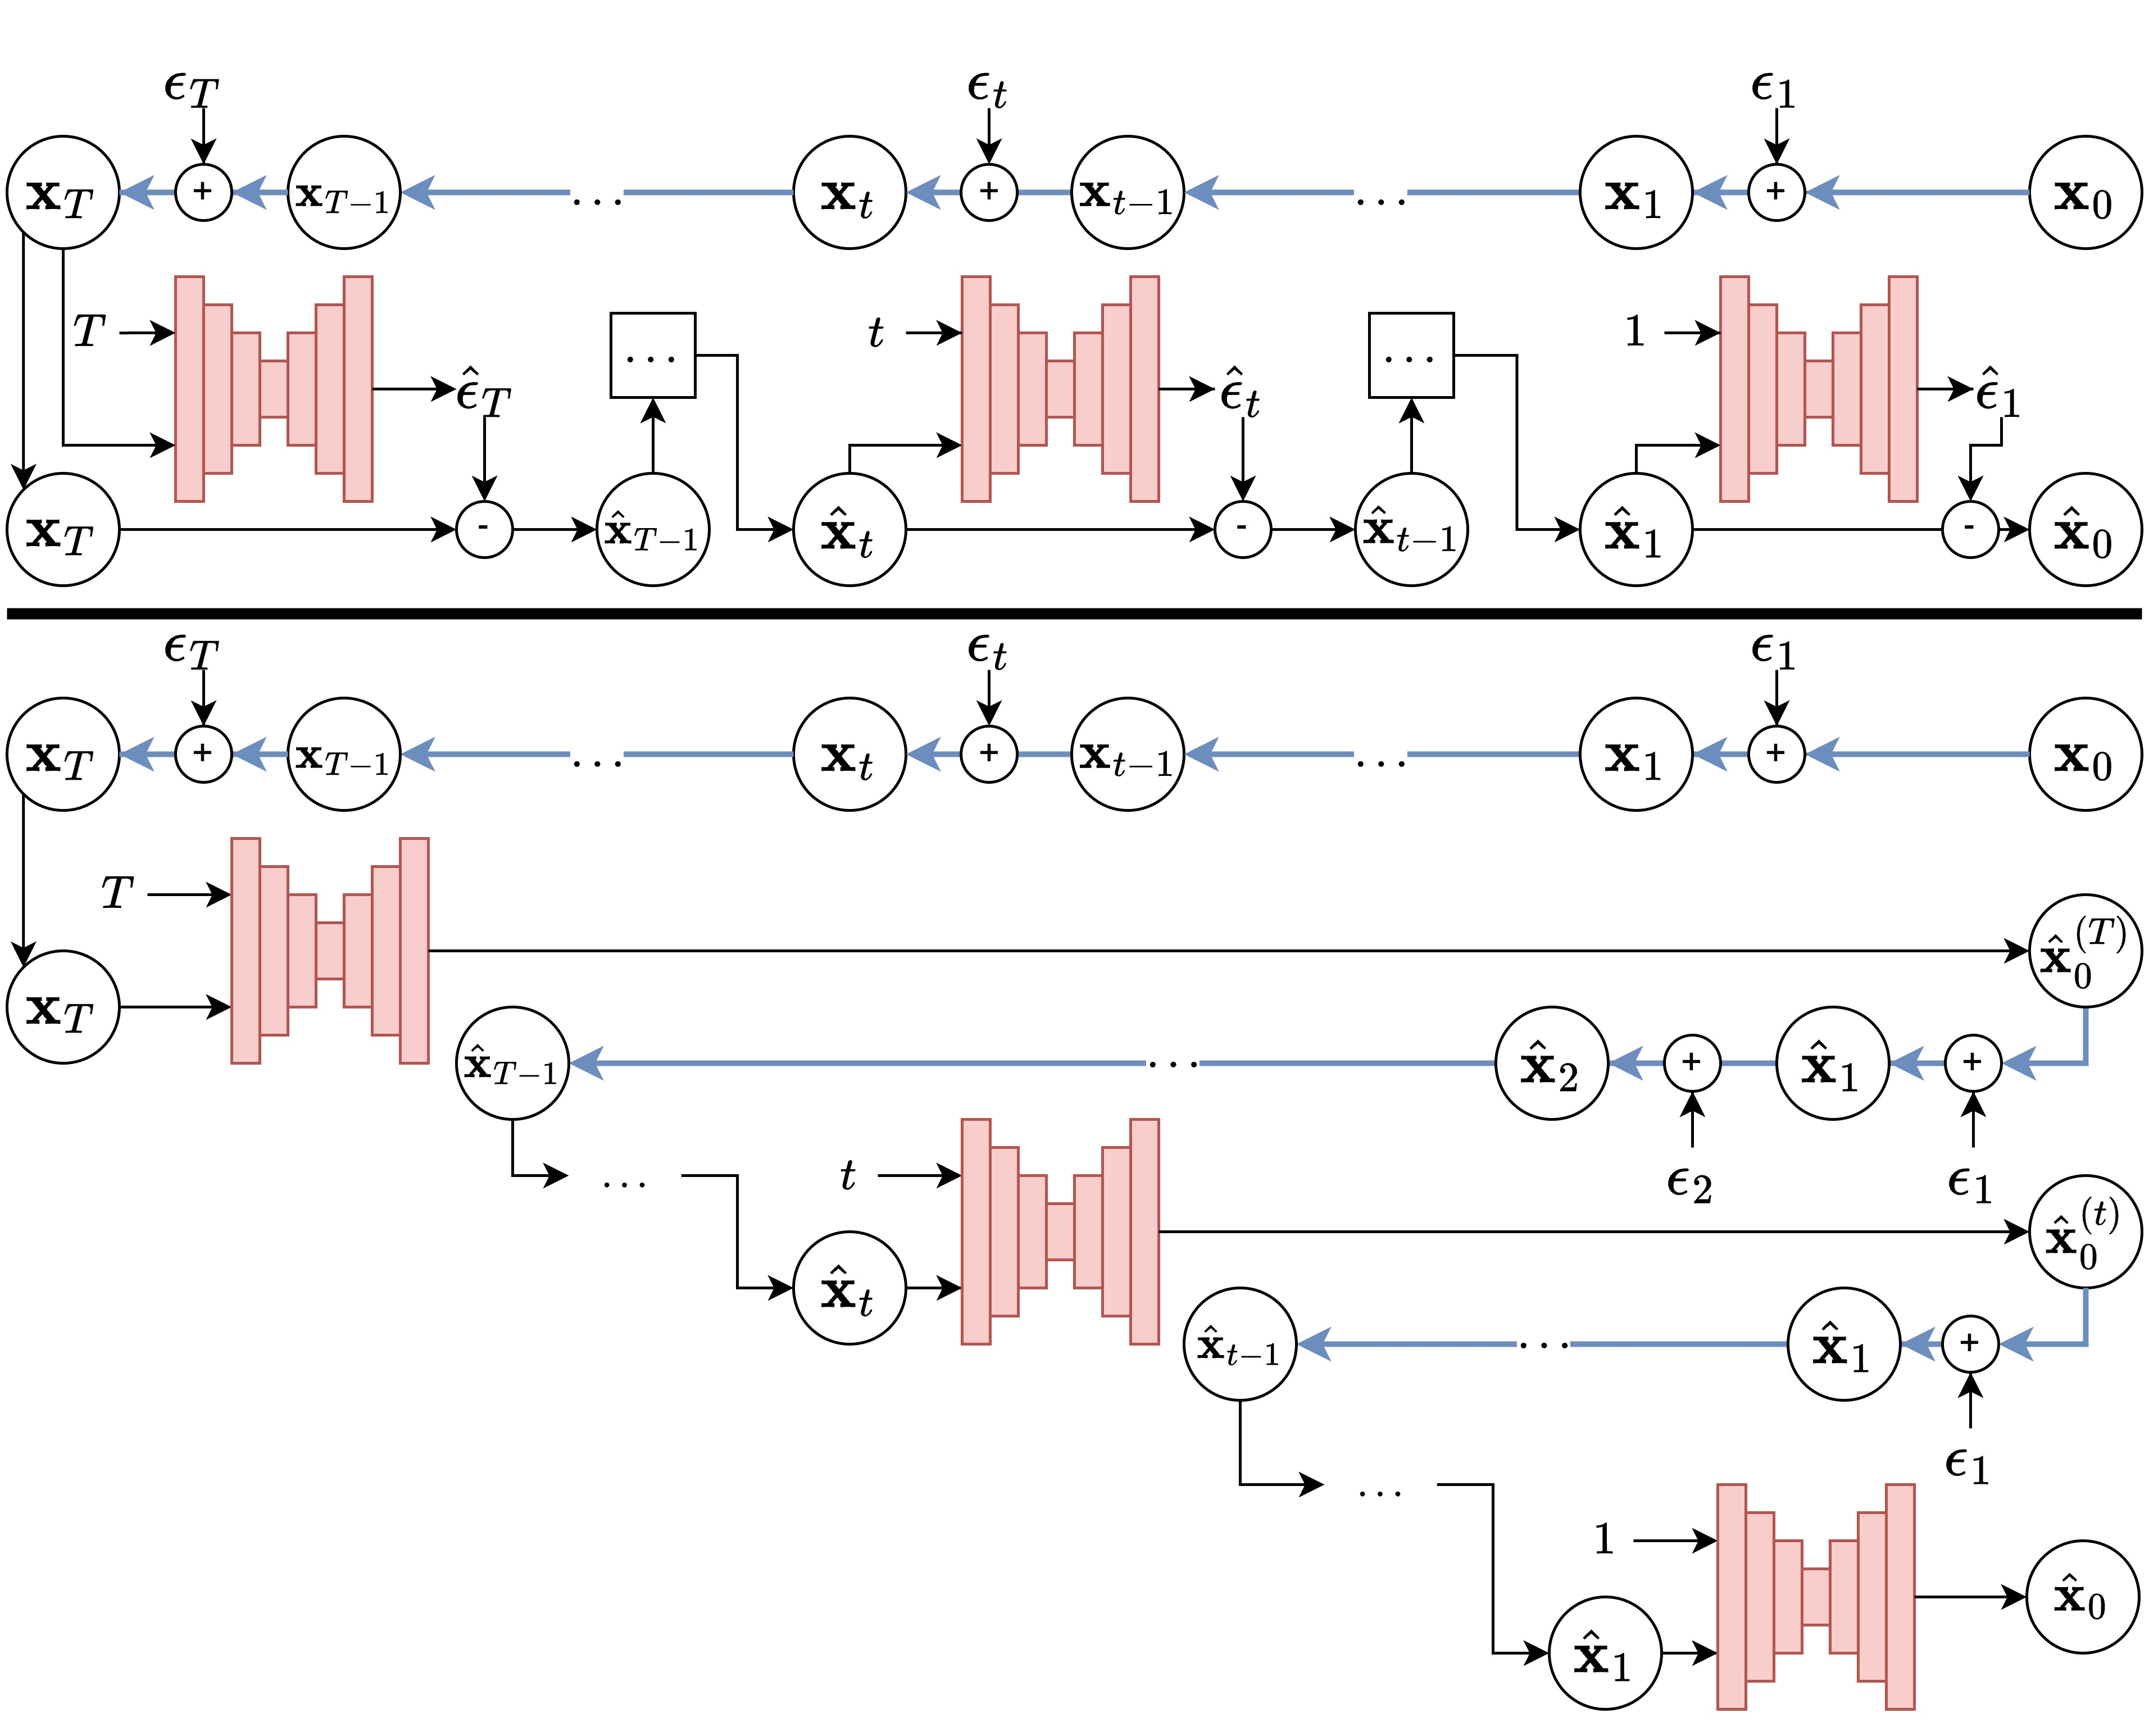
\includegraphics[width=\linewidth]{X0Objective}
	\label{fig:X0Objective}
	\caption{\textbf{So sánh $\epsilon$ objective (bên trên) và  $\bx_0$ (bên dưới)}. }
\end{figure}

\begin{itemize}
	\item \textbf{$\epsilon$  objective} :  mô hình sẽ dự đoán lỗi. Bắt đầu từ việc forward quá trình gây nhiễu để lấy được $\bx_T$, khi có được $\bx_T$ ta sẽ sử dụng $\bx_T \in \mathcal{N}(0, \mathbf{I})$ để đưa vào quá trình denoise. Trong quá trình denoise, mô hình sẽ dự đoán nhiễu $\hat{\epsilon}_t$ đã được thêm vào từ quá trình forward, là nhiễu $\epsilon_t$ và tối ưu lỗi giữa nhiễu dự đoán và nhiễu thực tế từ quá trình forward.
	\item \textbf{$\bx_0$ objective} : tương tự mô hình sẽ forward quá trình gây nhiễu để lấy được $\bx_T$, khi có được $\bx_T$ ta sẽ sử dụng $\bx_T \in \mathcal{N}(0, \mathbf{I})$ để đưa vào quá trình denoise. Mô hình sẽ dự đoán trực tiếp $\bx_0$, sau khi có $\bx_0$ mô hình sẽ tiếp tục gây nhiễu (Diffuse ) đến bước thứ $\bx_{t-1}$, và tiếp tục sử dụng $\bx_{t-1}$ để đưa vào mô hình dự đoán $\bx_0$
	\end{itemize}



%Praesent in sapien. Lorem ipsum dolor sit amet, consectetuer 
%adipiscing elit. Duis fringilla tristique neque. Sed interdum

%\begin{figure*}[p]
%	\centering
%	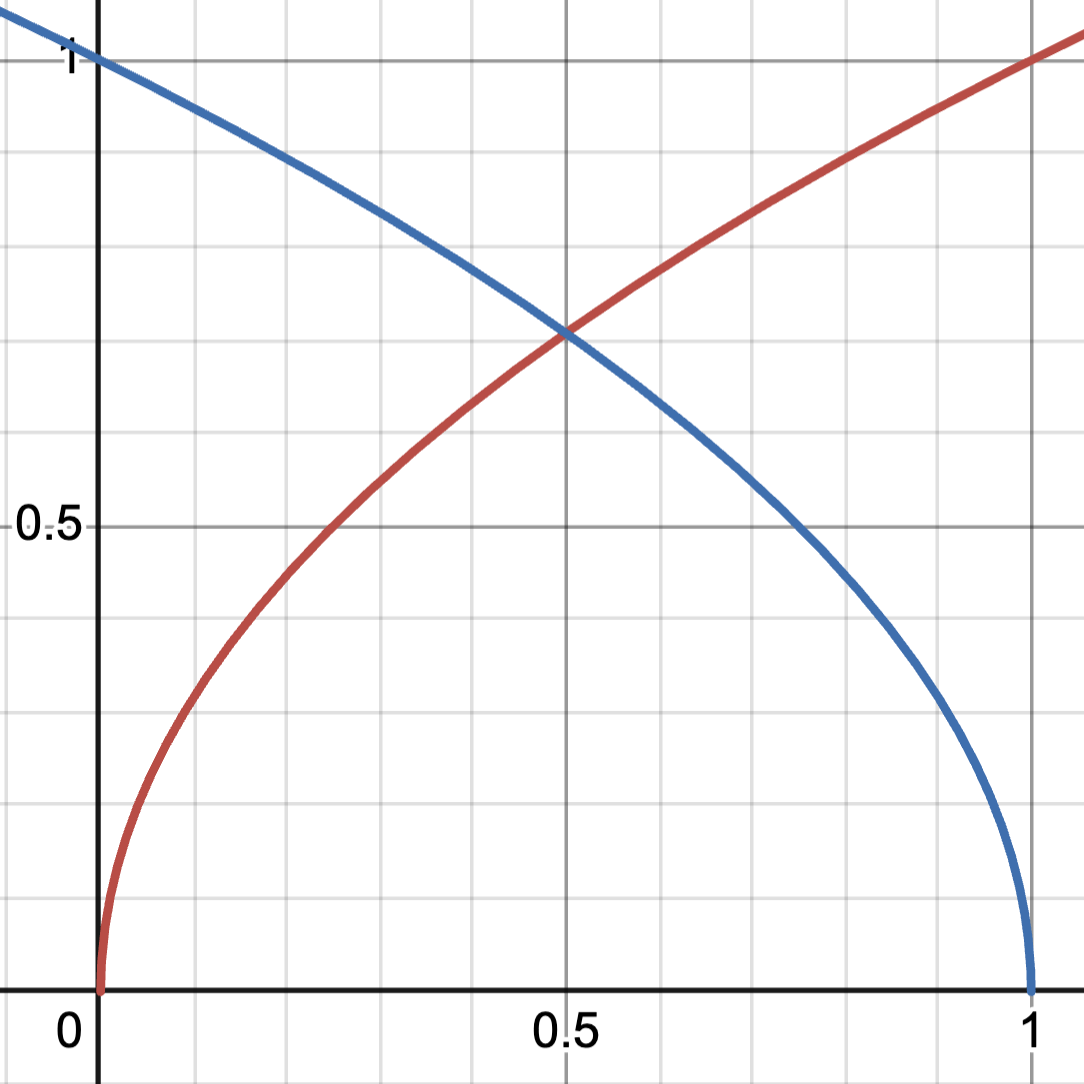
\includegraphics[width=0.5\linewidth]{images/beta_sqrtbeta}
%	\caption{Sự thay đổi của $\sqrt{\beta}$ và $\sqrt{1-\beta}$}
%	\label{fig:beta_sqrtbeta}
%\end{figure*}


%You can put more than one value in the parameter, for instance, if you write [ht] LaTeX will try to position the figure here, but if it's not possible (the space may be insufficient) then the figure will appear at the top of the page. It is recommended to use more than one positioning parameter to prevent unexpected results.
